\documentclass[tikz]{standalone}
\begin{document}

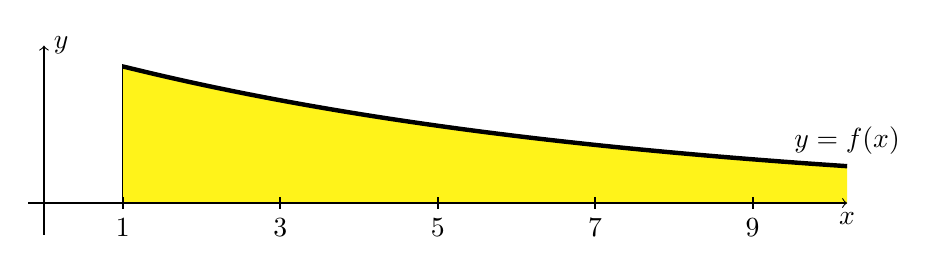
\begin{tikzpicture}[yscale=2]

  %shade region
  \fill[fill=yellow!90] plot[smooth, samples=100, domain=1:10.2 ] (\x,{2.71 ^ -(\x/7)})-- (10.2, 0) --(1, 0)-- cycle;
    
  %draw curve
  \draw[domain=1:10.2,smooth,variable=\x,black,ultra thick] plot ({\x},{2.71 ^ (-\x/7)}) 
        node[above]{$y=f(x)$};
    
  % tick marks
  \foreach \x in {1,3,...,9} 
    \draw [thick] (\x cm,1pt) -- (\x cm,-1pt) node[below] {$\x$};
  \foreach \y in {} 
    \draw [thick] (1pt,\y cm) -- (-1pt,\y cm) node[left] {$\y$};

  %draw axes
  \draw[->] (-0.2,0) -- (10.2,0) node[below] {$x$};
  \draw[->] (0,-0.2) -- (0,1) node[right] {$y$};

  \draw (1,0) -- (1,0.881);
\end{tikzpicture}
\end{document} 
